%\documentclass[a4paper,11pt]{article}
%\usepackage[T1]{fontenc}
%\usepackage[utf8]{inputenc}
%\usepackage{lmodern}
%\usepackage[french]{babel}
%\usepackage[squaren, Gray]{SIunits}
%\usepackage{circuitikz}
%\usepackage{graphicx}
%\usepackage{amsmath}
%\usepackage{amssymb}
%\usepackage{mathrsfs}
%\usepackage{subfigure}
%\usepackage[absolute]{textpos}
%\usepackage{url} 
%\usepackage[toc]{appendix}
%\usepackage{array}
%\usepackage[final]{pdfpages}
%\usepackage{listings}
%\usepackage[Lenny]{fncychap}
%\usepackage{multirow}
%\usepackage{ragged2e}
%\usepackage{verbatim}
%\usepackage[top=2cm, bottom=2cm, left=2cm, right=2cm]{geometry}
%\usepackage[rightcaption]{sidecap}
%\usepackage{listings}
%\usepackage{courier}
%\usepackage{color}

%\title{LINMA 2471: Optimization \\models and methods\\ }
%%\author{ Sebastion \bsc{Lagae} \and Arthur \bsc{Losseau}}
%\date{\today }
%
%\begin{document}
%\maketitle

\section{Introduction: AMPL}

AMPL (which stands for "A mathematical programming language") is an algebraic modelling language which enables the solving of high complexity problems for large (or small) scale models and will be used throughout this course. Knowing or identifying what type of problem we're dealing with is important and allows us to decide which will be the most adequate method to solve it. Certain methods work well with certain types of models, some are better than others, etc. \\

\begin{figure}[h!]
\centering
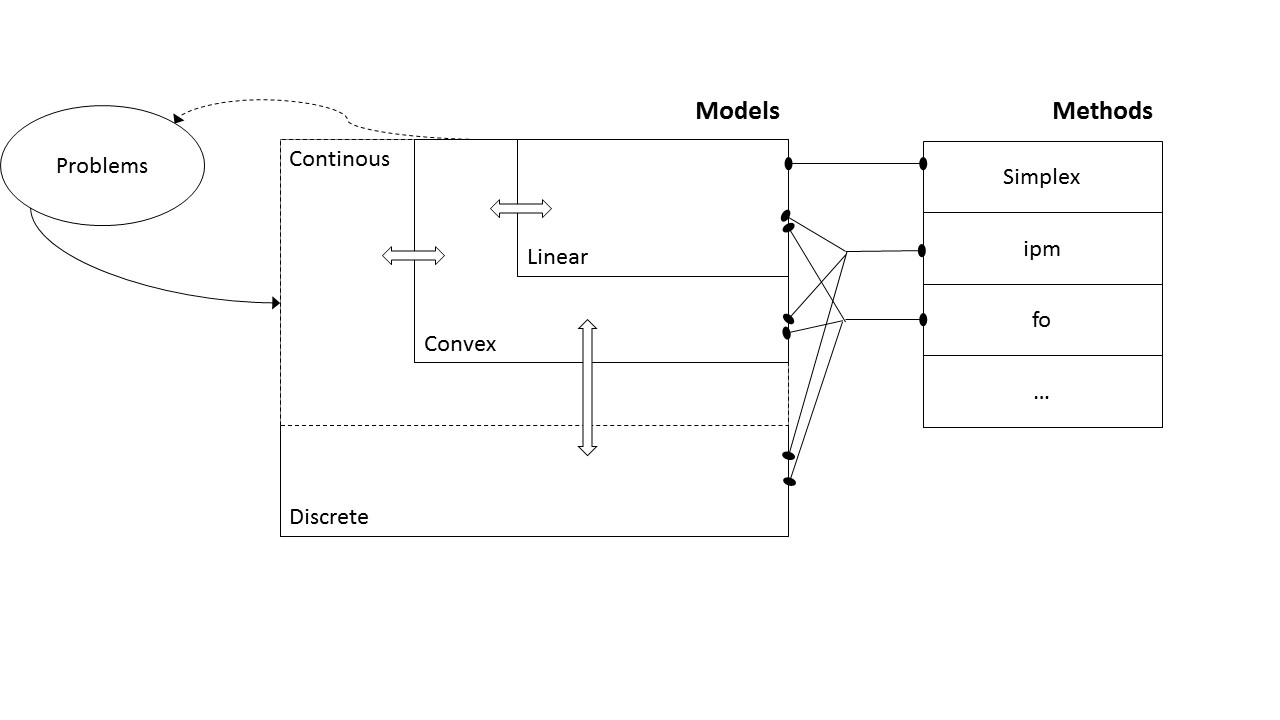
\includegraphics[width=\textwidth]{./images/Course1_Slide1.JPG}
\caption{Visualization of the relation between models and methods}
\label{Figure1}
\end{figure} 

AMPL works by first reading a text file which contains all the useful information of the model, this file usually ends in ".mod", it then parses it and tries to solve the problem. Parameters, variables, objective function and constraints are all defined in this file. The solving part is done by communicating with a solver, AMPL gives it all the information, the solver then sends back the solution. 
Consider the following optimization problem:

\begin{align*}
          &\min \, c^Tx  \\ 
       	 & Ay\le b\\
	 & l\le y\le u
\end{align*}
\\

For this problem AMPL will give the solver the usefull values ($c$,$A$,$b$,$l$,$u$,...) it neads to solve the problem. There exists quite a few of these solvers, some mode adapted to certain model types (linear, convex,...). 
We have for example:

\begin{itemize}
  \item minos (basic solver for linear and nonlinear problems)
  \item cplex (can be used for linear, convex, mixted integer models)
  \item gurobi (very similar to cplex)
  \item knitro (good for nonlinear models)
  \item $\cdots$
\end{itemize} 

This can be summerized by the next table: 

\begin{tabular}{|C{0.2 \textwidth}|L{0.5 \textwidth}|C{0.2 \textwidth}|}
\hline
Solvers & Problems & Integer variables \\
\hline
\hline
CPLEX, GUROBI & linear optimization and convex quadratic optimization & yes \\
\hline
KNITRO, SNOPT, MINOS & nonlinear optimization & yes for KNITRO but loss of efficiency \\
\hline
BARON & global optimization & no \\
\hline
\end{tabular}

\begin{figure}[h!]
\centering
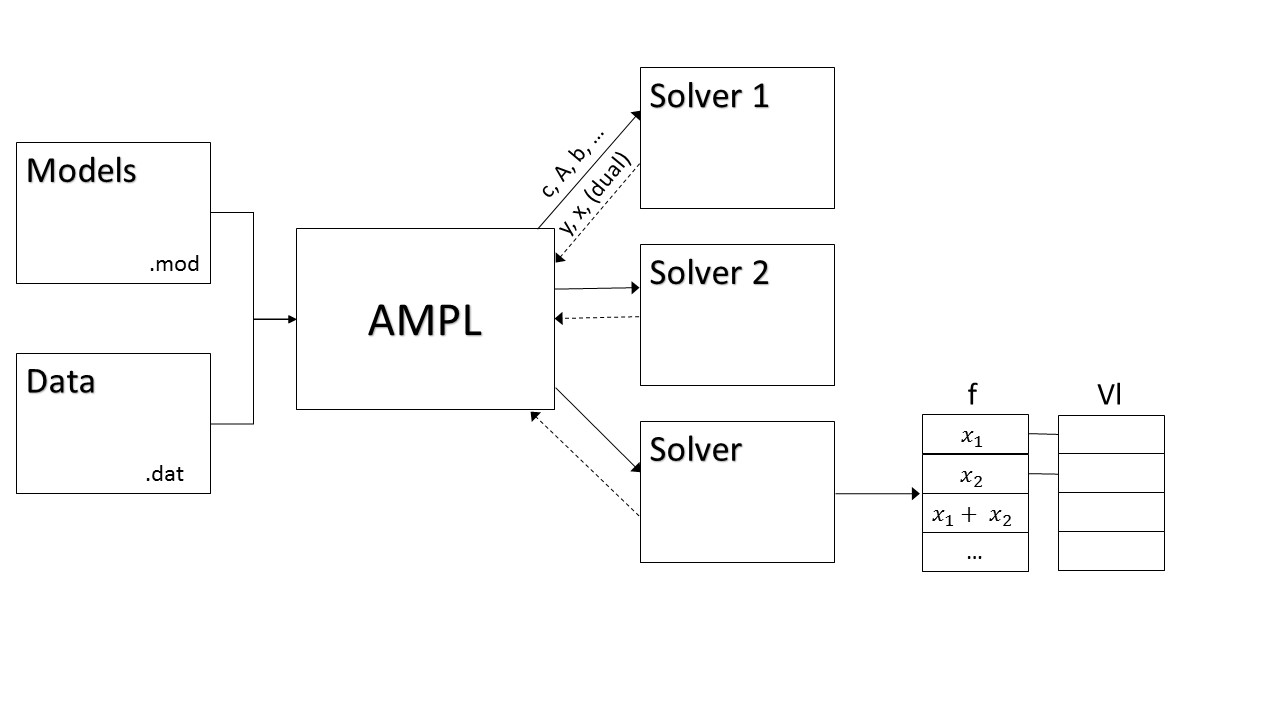
\includegraphics[width=\textwidth]{./images/Course1_Slide2.JPG}
\caption{}
\label{Figure2}
\end{figure} 

AMPL can also work with an additionnal data file (".dat") which is used when parameters are left in the model file. This allows us to avoid changing the entire file when looking at different values of parameters, and only having to change them once in the data file. \\

A few examples and the basic syntax for AMPL can be found in the Tutorials Dropbox, given on Moodle. \\

Everything in AMPL has a name, whether it be variables, constants, or even constraints (which represent a dual variable) and each command and declaration ends with a semicolon (";"). 
Certain commands are worth being reminded here, for example: \\

\begin{itemize}
  \item Changing solvers: \textbf{option solver ... ;}
  \item Displaying dual variable: \textbf{display Protein;}
  \item Displaying variable: \textbf{display Protein.body;}
  \item Reset the whole model: \textbf{reset;}
  \item Chosing a model file: \textbf{data data1.dat;}
  \item Chosing a data file: \textbf{model data1.mod;}
  \item Solving the chosen model: \textbf{solve;}
\end{itemize} 



